%% =====================================================================
%%  INFORME DE LABORATORIO - PRÁCTICA DE DUREZA (formato IEEE)
%%  Ciencia e Ingeniería de Materiales - Universidad Nacional de Colombia
%%  Compilar con pdfLaTeX (2 pasadas para resolver citas y referencias).
%%  Las imágenes van en la carpeta  Figuras/  (mismo nivel que este .tex).
%%  Lo que aparece en ROJO (macro \vf) falta o debe confirmarse. Cuando
%%  todo esté resuelto, para quitar el rojo basta con cambiar la línea
%%  \newcommand{\vf}...  de abajo por:  \newcommand{\vf}[1]{#1}
%% =====================================================================
\documentclass[journal,11pt]{IEEEtran}

\usepackage[utf8]{inputenc}
\usepackage[T1]{fontenc}
\usepackage[spanish,es-tabla,es-noquoting]{babel}
\usepackage{amsmath,amssymb}
\usepackage{graphicx}
\usepackage{booktabs}
\usepackage{array}
\usepackage{siunitx}
\usepackage{xcolor}
\usepackage{tikz}
\usetikzlibrary{babel,arrows.meta,positioning,calc}
\usepackage{pgfplots}
\usepgfplotslibrary{groupplots}
\pgfplotsset{compat=1.16}
\usepackage{cite}

\graphicspath{{./}{./Figuras/}}

% --- Ajustes de siunitx (coma decimal) y unidades propias ---
\sisetup{output-decimal-marker={,}, group-digits=false}
\DeclareSIUnit\kgf{kgf}
\DeclareSIUnit\gf{gf}

% --- Rótulos en español (estilo IEEE) ---
\addto\captionsspanish{%
  \def\figurename{Fig.}%
  \def\tablename{Tabla}%
  \def\abstractname{Resumen}%
  \def\IEEEkeywordsname{Palabras clave}}

% --- Marca en rojo lo que hay que confirmar o completar ---
\newcommand{\vf}[1]{{\color{red}#1}}

\begin{document}

\title{Ensayos de dureza Rockwell y microdureza Knoop en acero y cobre:
calibración, selección de escala y conversión entre métodos\\[3pt]
\large\textit{Rockwell and Knoop Hardness Testing of Steel and Copper:
Calibration, Scale Selection and Method Conversion}}

\author{%
\IEEEauthorblockN{Juan José Tobar Álvarez, Angélica Plata Martínez, Sergio Correales Sarmiento,\\
Nombre Apellido 4 y Nombre Apellido 5}
\IEEEauthorblockA{Universidad Nacional de Colombia, Sede Bogotá --- Facultad de Ingeniería\\
Departamento de Ingeniería Mecánica y Mecatrónica\\
Ciencia e Ingeniería de Materiales (2017256-1), Grupo~01\\
Prof. Jhon Jairo Olaya Flórez --- Práctica de dureza, 21 de octubre de 2026\\
jutobara@unal.edu.co, anplatam@unal.edu.co, scorreales@unal.edu.co}}

\maketitle

% ---------------------------------------------------------------------
\begin{abstract}
Se determinó la dureza de un acero endurecido y de cobre mediante ensayos Rockwell y de microdureza Knoop, y se evaluó cómo la selección de la escala condiciona la validez de la medición. Los ensayos Rockwell se hicieron en un durómetro analógico manual Wolpert HT~2000 (precarga de 10~kgf), previa verificación con un patrón de $\approx$20~HRC (cuatro ensayos); la microdureza se midió en un equipo LECO LM~110 con indentador Knoop, carga de 500~gf y 10~s de aplicación sobre una probeta empastillada en baquelita. La verificación arrojó un promedio de 19,98~HRC (error de $-0{,}03$~HRC; desviación estándar de 0,82~HRC). El acero presentó $65{,}3\pm0{,}5$~HRC (IC del 95~\%, $n=6$; CV~=~0,7~\%), equivalente a $\approx$832~HV según la carta de conversión. En el cobre, la escala C resultó inadecuada (la aguja dio $\approx$2,5 vueltas), la escala B quedó cerca del límite inferior (22,2~HRB) y la escala F, apropiada, entregó $71{,}8\pm2{,}0$~HRF ($n=6$; CV~=~2,7~\%). La huella Knoop, con diagonal mayor de 120,2~\textmu m, correspondió a 492~HK~0,5 ($\approx$4,8~GPa), consistente con los $\approx$47~HRC rotulados en la probeta. Se concluye que la escala debe elegirse según la dureza esperada, que el equipo analógico fue exacto en promedio pero con dispersión apreciable, y que las conversiones entre escalas son aproximadas y válidas solo dentro de una misma familia de materiales.
\end{abstract}

\begin{IEEEkeywords}
acero, calibración, cobre, conversión de escalas, dureza, microdureza Knoop, Rockwell.
\end{IEEEkeywords}

% =====================================================================
\section{Introducción y objetivos}
\IEEEPARstart{L}{a} dureza se define como la resistencia de un material a la deformación plástica localizada, y se mide forzando un indentador de geometría conocida contra su superficie \cite{callister,ashby}. Es una de las propiedades mecánicas más utilizadas en ingeniería porque el ensayo es rápido, económico y prácticamente no destructivo, y porque se correlaciona con la resistencia a la fluencia: en metales con bajo endurecimiento por deformación, la dureza es del orden de tres veces el límite elástico \cite{tabor}. Por ello se emplea en el control de calidad de tratamientos térmicos, en la verificación de lotes y en la selección de materiales \cite{asmhb}.

Los métodos de uso más extendido son Brinell, Vickers, Knoop y Rockwell. El método Rockwell \cite{astm18,iso6508} determina la dureza a partir de la profundidad permanente que deja un penetrador al aplicar y retirar una carga, por lo que es directo y adecuado para producción; la microdureza Knoop \cite{astm384,iso4545,knoop} utiliza cargas de gramos y relaciona la carga con el tamaño de la huella, lo que permite medir zonas muy pequeñas, capas delgadas o fases individuales. El campo de la indentación abarca desde la macrodureza hasta la nanodureza \cite{broitman}. Un aspecto crítico es que el resultado solo es válido si la escala, el penetrador y la carga son los adecuados para la dureza del material.

Esta práctica se desarrolló el 21 de octubre de 2026 en el Laboratorio de Metalografía de la Universidad Nacional de Colombia, Sede Bogotá, con apoyo del texto de laboratorio del curso \cite{forero}. Su aporte es mostrar, con un acero endurecido y con cobre, cómo la elección de la escala determina la validez de la medición, y cómo se cuantifican la exactitud y la dispersión de un durómetro mediante un patrón y un tratamiento estadístico sencillo.

\textbf{Objetivo general.} Determinar la dureza de un acero y de cobre mediante los métodos Rockwell y de microdureza Knoop, evaluando el efecto de la selección de la escala y la calidad de la medición.

\textbf{Objetivos específicos:}
\begin{enumerate}
\item Seleccionar el penetrador, la escala y la carga según la dureza esperada de cada material.
\item Verificar el durómetro Rockwell con un patrón y calcular el error de la medición.
\item Medir la dureza del acero y del cobre y analizar estadísticamente los resultados.
\item Calcular la microdureza Knoop a partir de la diagonal de la huella obtenida con 500~gf.
\item Comparar los resultados entre escalas con la carta de conversión y discutir sus limitaciones.
\end{enumerate}

% =====================================================================
\section{Fundamentos teóricos}
\subsection{Ensayo Rockwell}
En el ensayo Rockwell \cite{astm18,iso6508} el penetrador se apoya sobre la probeta con una precarga $F_0=\SI{10}{\kgf}$ ($\SI{98,07}{\newton}$), que elimina el efecto de la rugosidad y fija la referencia de profundidad; luego se añade la carga adicional $F_1$ hasta alcanzar la carga total $F=F_0+F_1$, se retira $F_1$ y, con la precarga aún aplicada, se lee el incremento permanente de profundidad $e$ (Fig.~\ref{fig:principio}). El número de dureza es
\begin{equation}
\mathrm{HR}=N-\frac{e}{\SI{0,002}{\milli\metre}},
\label{eq:rockwell}
\end{equation}
con $N=100$ para penetradores de diamante y $N=130$ para bola de acero; cada unidad Rockwell equivale a \SI{0,002}{\milli\metre} y una vuelta completa de la aguja grande, a 100 unidades (\SI{0,2}{\milli\metre}). La escala depende de la combinación penetrador--carga (Tabla~\ref{tab:escalas}); las escalas de diamante se leen en la escala negra de la carátula y las de bola, en la roja. Como regla práctica, para materiales duros se usa un cono de diamante de $120^{\circ}$ (escalas A y C) y para materiales blandos una bola de 1/16~in (escalas B y F); el diamante en forma de pirámide corresponde al método Vickers. En la práctica industrial actual la bola es de carburo de tungsteno \cite{iso6508}, mientras que en el equipo del laboratorio es de acero templado.

\begin{figure}[!t]
\centering
\begin{tikzpicture}[font=\scriptsize,>={Stealth[length=1.6mm]},
  lab/.style={anchor=west,align=left,text width=4.7cm}]
\fill[gray!20] (0,-3.3) rectangle (2.9,0);
\draw[thick] (-0.3,0) -- (3.2,0);
\node[anchor=south west] at (-0.3,0.02) {Superficie de la probeta};
\draw[dashed] (0,-0.7) -- (3.2,-0.7);
\node[lab] at (3.25,-0.7) {(1) Precarga $F_0$: fija el cero (profundidad $h_0$)};
\draw[dashed] (0,-1.75) -- (3.2,-1.75);
\node[lab] at (3.25,-1.75) {(3) Se retira $F_1$ con $F_0$ aplicada: profundidad $h_2$ y lectura de $e$};
\draw[dashed] (0,-2.6) -- (3.2,-2.6);
\node[lab] at (3.25,-2.6) {(2) Carga total $F=F_0+F_1$: profundidad $h_1$};
\draw[<->] (1.45,-0.7) -- (1.45,-1.75) node[midway,right] {$e=h_2-h_0$};
\end{tikzpicture}
\caption{Principio del ensayo Rockwell: la dureza se obtiene de la profundidad permanente $e$ medida respecto a la posición con precarga.}
\label{fig:principio}
\end{figure}

\begin{table}[!t]
\caption{Escalas Rockwell consideradas en la práctica.}
\label{tab:escalas}
\centering\footnotesize
\begin{tabular}{@{}llcc>{\raggedright\arraybackslash}p{2.2cm}@{}}
\toprule
Escala & Penetrador & $F$ (kgf) & Rango & Aplicación típica\\
\midrule
HRA & Cono $120^{\circ}$ & 60 & 20--88 & Muy duros; láminas delgadas y duras\\
HRB & Bola 1/16 in & 100 & 20--100 & Aceros blandos, Cu y Al\\
HRC & Cono $120^{\circ}$ & 150 & 20--70 & Aceros endurecidos\\
HRF & Bola 1/16 in & 60 & 60--100 & Cobre recocido, láminas\\
\bottomrule
\end{tabular}
\end{table}

Para que la lectura sea válida, la probeta debe tener caras planas y paralelas, estar libre de óxido, grasa y pintura, tener un espesor de al menos diez veces la profundidad permanente $e$ (quince veces con penetrador esférico en ISO~6508-1) y recibir huellas separadas por al menos tres diámetros entre centros y $2{,}5$ diámetros del borde \cite{astm18,iso6508}. Los valores fuera del rango de cada escala (Tabla~\ref{tab:escalas}) se consideran poco confiables, y sobre superficies convexas es necesario aplicar correcciones \cite{astm18}. Además, el equipo debe verificarse con bloques patrón y cada vez que se cambia la carga se repite la verificación y se calcula el error respecto al valor nominal.

\subsection{Microdureza Knoop}
El indentador Knoop es una pirámide de diamante de base romboidal cuyos ángulos en los planos de las diagonales son $172^{\circ}30'$ y $130^{\circ}$, de modo que la diagonal mayor $d$ es $\approx7{,}11$ veces la menor y la profundidad es $\approx d/30{,}5$ \cite{knoop,astm384}. La dureza se calcula como la relación entre la carga $P$ y el área proyectada de la huella:
\begin{equation}
\mathrm{HK}=\frac{P}{A_p}=\frac{\num{14.229}\,P}{d^{2}},
\label{eq:knoop}
\end{equation}
donde $P$ se expresa en kgf y $d$ en mm (HK en kgf/mm$^2$). Se reporta como, por ejemplo, 492~HK~0,5, donde 0,5 es la carga en kgf. Al medirse solo la diagonal mayor, que apenas se recupera elásticamente, el método es poco sensible a la recuperación elástica y apto para materiales frágiles y capas delgadas; la norma aplica a diagonales mayores de al menos \SI{20}{\micro\metre} \cite{iso4545}. Los resultados requieren superficie plana, paralela y pulida a espejo (en la práctica, lijado hasta grano 600 y paño), así como un tiempo de aplicación de la carga de 10 a 15~s \cite{astm384}.

\subsection{Conversión entre escalas}
Las conversiones entre Rockwell, Vickers, Knoop y Brinell son empíricas y válidas solo para la familia de materiales con que se construyeron; por eso la norma ASTM~E140 presenta tablas separadas, por ejemplo para aceros no austeníticos, aleaciones de níquel, latón de cartucho, cobre y aluminio forjado, y advierte que los valores son aproximados \cite{astm140}. En la práctica se usan cartas como la del laboratorio \cite{leco}.

\subsection{Tratamiento estadístico}
Para $n$ lecturas $x_i$ se calcularon el promedio $\bar{x}$, la desviación estándar muestral $s$, el coeficiente de variación $\mathrm{CV}$, el intervalo de confianza del 95~\% para la media (incertidumbre tipo~A \cite{gum}) y el error respecto del valor nominal $x_{nom}$ de un patrón:
\begin{align}
\bar{x}&=\frac{1}{n}\sum_{i=1}^{n}x_i, \qquad
s=\sqrt{\frac{\sum_{i=1}^{n}(x_i-\bar{x})^2}{n-1}}, \label{eq:stat1}\\
\mathrm{CV}&=\frac{s}{\bar{x}}\times100, \qquad
\mathrm{IC}_{95}=\bar{x}\pm t_{0{,}975,\,n-1}\frac{s}{\sqrt{n}}, \label{eq:stat2}\\
E&=\bar{x}-x_{nom}. \label{eq:error}
\end{align}

% =====================================================================
\section{Metodología experimental}
\subsection{Materiales y equipos}
Se ensayaron tres probetas (Fig.~\ref{fig:anexo2}): un disco plano de acero endurecido (``Acero~1'', de composición y tratamiento desconocidos; dimensiones no medidas durante la sesión), una barra rectangular de cobre (sección no medida durante la sesión) y una probeta de acero 1045 empastillada en baquelita para microdureza, rotulada ``1045, austenizado 850~\si{\degreeCelsius}/30~min, austemperado 200~\si{\degreeCelsius}/90~min, 47~HRC''. Los equipos se esquematizan en la Fig.~\ref{fig:equipos}:
\begin{itemize}
\item \textbf{Durómetro Rockwell Wolpert (Amsler Otto Wolpert-Werke GmbH), tipo HT~2000}, construido en 1984 (220~V, 0,31~A, 60~Hz), de accionamiento manual, con precarga de \SI{10}{\kgf}, cargas totales seleccionables mediante pasadores laterales (15,625 a \SI{250}{\kgf}), tiempo de aplicación de la carga no ajustable (10~s como valor de referencia general indicado en el laboratorio; en la operación manual, la permanencia bajo carga total fue de $\approx$\SI{3}{\second}) y carátula analógica con escalas negra (diamante) y roja (bola de acero templado de 1/16~in).
\item \textbf{Microdurómetro LECO LM~110} (placa: serie FMS1257), con ocular WF10X con retículo y dos tambores micrométricos laterales, objetivos para aumentos de 100$\times$ y 500$\times$, platina X--Y con micrómetros, iluminación regulable y carga seleccionable entre \SI{10}{\gf} y \SI{1}{\kgf}, equipado con indentador Knoop de diamante.
\end{itemize}
Las condiciones ambientales del laboratorio, leídas en un termohigrómetro, fueron de $\approx$\SI{20}{\degreeCelsius} y 55--58~\% de humedad relativa, dentro del intervalo de 10 a \SI{35}{\degreeCelsius} que fija ASTM~E18 para ensayos Rockwell \cite{astm18}.

\begin{figure*}[!t]
\centering
\begin{minipage}[b]{0.31\textwidth}\centering
\resizebox{\linewidth}{!}{%
\begin{tikzpicture}[every node/.style={font=\scriptsize}]
% base, columna y brazo
\draw[fill=gray!20] (0,0) rectangle (5.4,1.1);
\draw[fill=gray!20] (0,1.1) -- (0,7) -- (4.2,7) -- (4.2,5.7) -- (1,5.7) -- (1,1.1) -- cycle;
% carátula
\draw[fill=brown!40] (2.7,5.7) rectangle (4.2,7);
\draw[fill=white] (3.45,6.35) circle (0.45);
\draw (3.45,6.35) -- (3.58,6.72);
% penetrador
\draw[fill=black] (3.37,5.7) rectangle (3.53,5.3);
\fill[black] (3.37,5.3) -- (3.45,4.98) -- (3.53,5.3) -- cycle;
% probeta, yunque, tornillo con fuelle, volante
\draw[fill=blue!15] (2.4,4.55) rectangle (4.5,4.98);
\draw[fill=gray!60] (2.0,4.25) rectangle (4.9,4.55);
\draw[fill=black!70] (2.9,2.6) rectangle (4.0,4.25);
\draw[fill=gray!40] (3.45,2.35) ellipse (1.3 and 0.28);
\draw[fill=gray!60] (2.9,1.1) rectangle (4.0,2.1);
% selector de carga (lado izquierdo)
\draw[fill=brown!60] (-0.5,3.0) rectangle (0,5.4);
\foreach \y in {3.2,3.5,3.8,4.1,4.4,4.7,5.0,5.25} \draw[line width=1.8pt] (-0.5,\y) -- (-0.9,\y);
% numeración
\foreach \n/\x/\y/\ex/\ey in {1/4.2/6.35/5.9/6.35, 2/3.55/5.2/5.9/5.2, 3/4.5/4.76/5.9/4.76,
  4/4.9/4.4/5.9/4.4, 5/4.0/3.4/5.9/3.4, 6/4.75/2.35/5.9/2.35, 7/-0.9/4.2/-1.5/4.2, 8/0/6.4/-1.5/6.4}
 {\draw[thin] (\x,\y) -- (\ex,\ey); \node[circle,draw,fill=white,inner sep=0.8pt] at (\ex,\ey) {\n};}
\end{tikzpicture}}\\[2pt]
(a)
\end{minipage}\hfill
\begin{minipage}[b]{0.31\textwidth}\centering
\resizebox{\linewidth}{!}{%
\begin{tikzpicture}[every node/.style={font=\scriptsize}]
% base y panel de control
\draw[fill=gray!20] (0,0) rectangle (5.4,1.6);
\draw[fill=gray!60] (2.6,0.25) rectangle (5.0,1.35);
\fill[green!60!black] (2.8,1.1) circle (0.07);
\draw[fill=black] (3.6,0.55) rectangle (4.0,0.8);
\draw[fill=black] (4.15,0.55) rectangle (4.55,0.8);
% columna y brazo
\draw[fill=gray!20] (0,1.6) -- (0,6.4) -- (4.2,6.4) -- (4.2,5.2) -- (1.1,5.2) -- (1.1,1.6) -- cycle;
% ocular
\draw[fill=black!80] (3.2,6.4) rectangle (4.6,7.0);
\draw[fill=black!80] (4.6,6.55) rectangle (5.0,6.85);
% objetivo e indentador
\draw[fill=black!70] (3.0,4.75) rectangle (3.5,5.2);
\draw[fill=black] (3.65,4.8) rectangle (3.85,5.2);
\fill[black] (3.65,4.8) -- (3.75,4.5) -- (3.85,4.8) -- cycle;
% probeta (baquelita), platina X-Y, micrómetro, pilar
\draw[fill=red!40!black!60] (3.2,4.1) rectangle (4.4,4.45);
\draw[fill=black!70] (2.3,3.7) rectangle (5.2,4.1);
\draw[fill=gray!50] (5.2,3.75) rectangle (5.9,4.05);
\draw[fill=gray!60] (3.0,1.6) rectangle (3.9,3.7);
% numeración
\foreach \n/\x/\y/\ex/\ey in {1/5.0/6.7/6.3/6.7, 3/3.85/5.0/6.3/5.0, 4/4.4/4.28/6.3/4.28,
  5/5.9/3.9/6.3/3.5, 7/5.0/0.8/6.3/0.8, 2/3.0/4.95/2.4/4.95, 6/3.0/2.6/2.2/2.6}
 {\draw[thin] (\x,\y) -- (\ex,\ey); \node[circle,draw,fill=white,inner sep=0.8pt] at (\ex,\ey) {\n};}
\end{tikzpicture}}\\[2pt]
(b)
\end{minipage}\hfill
\begin{minipage}[b]{0.31\textwidth}\centering
\resizebox{\linewidth}{!}{%
\begin{tikzpicture}[every node/.style={font=\large}]
\draw[thick, fill=gray!15] (-3.5,0) -- (0,0.49) -- (3.5,0) -- (0,-0.49) -- cycle;
\draw[dashed] (-3.5,0) -- (3.5,0);
\draw[dashed] (0,-0.49) -- (0,0.49);
\draw[{Stealth[length=2mm]}-{Stealth[length=2mm]}] (-3.5,-1.1) -- (3.5,-1.1) node[midway,below] {$d$ (diagonal mayor)};
\draw[{Stealth[length=2mm]}-{Stealth[length=2mm]}] (4.0,-0.49) -- (4.0,0.49);
\node[anchor=west] at (4.1,0) {$b\approx d/7{,}11$};
\node at (0,1.35) {$\alpha=172^{\circ}30'$ (plano de $d$)};
\node at (0,1.85) {$\beta=130^{\circ}$ (plano de $b$)};
\node at (0,-2.3) {Profundidad $\approx d/30{,}5$};
\end{tikzpicture}}\\[2pt]
(c)
\end{minipage}
\caption{Esquemas de los equipos. (a) Durómetro Rockwell Wolpert HT~2000: 1) carátula, 2) penetrador, 3) probeta, 4) yunque, 5) tornillo elevador con fuelle, 6) volante, 7) selector de carga, 8) bastidor. (b) Microdurómetro LECO LM~110: 1) ocular, 2) objetivo, 3) indentador, 4) probeta empastillada, 5) platina X--Y con micrómetros, 6) pilar, 7) panel de control. (c) Geometría de la huella Knoop.}
\label{fig:equipos}
\end{figure*}

\subsection{Procedimiento}
La secuencia general se resume en la Fig.~\ref{fig:flujo} y los parámetros de los ensayos Rockwell, en la Tabla~\ref{tab:param}. Las mediciones se hicieron bajo la guía del técnico del laboratorio y siguiendo sus normas de seguridad (uso obligatorio de bata de laboratorio u overol).

\begin{figure}[!t]
\centering
\begin{tikzpicture}[node distance=0.32cm, every node/.style={font=\scriptsize},
 box/.style={draw, rounded corners=2pt, align=center, text width=7.4cm, minimum height=0.6cm, fill=gray!8},
 arr/.style={-{Stealth[length=2mm]}, thick}]
\node[box] (a) {Preparación de probetas: caras planas y paralelas; lija 220 (Rockwell; no aplicada a la barra de cobre) o hasta 600 y paño (microdureza)};
\node[box, below=of a] (b) {Selección de escala: material duro $\rightarrow$ HRC; material blando $\rightarrow$ HRB/HRF};
\node[box, below=of b] (c) {Verificación con patrón $\approx$20~HRC (escala negra, precarga 10~kgf): 4 ensayos, promedio y error};
\node[box, below=of c] (d) {Acero: 6 ensayos HRC (150~kgf)};
\node[box, below=of d] (e) {Cobre: HRC (150~kgf), HRB (100~kgf) y 6 ensayos HRF (60~kgf)};
\node[box, below=of e] (f) {Microdureza Knoop: 500~gf, 10~s; medición de la diagonal mayor (2 lecturas)};
\node[box, below=of f] (g) {Cálculo de HK, estadística (promedio, $s$, CV, IC 95~\%) y conversión de escalas};
\foreach \p/\q in {a/b,b/c,c/d,d/e,e/f,f/g} \draw[arr] (\p) -- (\q);
\end{tikzpicture}
\caption{Diagrama de flujo del procedimiento experimental.}
\label{fig:flujo}
\end{figure}

\begin{table}[!t]
\caption{Parámetros de los ensayos Rockwell. Precarga de 10~kgf (98,07~N) y permanencia bajo carga total de $\approx$3~s en todos los casos (referencia general del laboratorio: 10~s); 150, 100 y 60~kgf equivalen a 1471, 981 y 588~N.}
\label{tab:param}
\centering\footnotesize
\begin{tabular}{@{}p{1.55cm}p{1.0cm}p{2.3cm}p{1.0cm}@{}}
\toprule
Parámetro & Acero & Cobre & Patrón\\
\midrule
Escala & HRC & HRC, HRB, HRF & HRC\\
Penetrador & Cono & Cono (C); bola (B, F) & Cono\\
Carga total (kgf) & 150 & 150; 100; 60 & 150\\
N.º de ensayos & 6 & 1; 1; 6 & 4\\
Escala del dial & Negra & Negra (C); roja (B, F) & Negra\\
\bottomrule
\end{tabular}
\end{table}

\begin{enumerate}
\item \textbf{Preparación.} Las probetas deben tener caras planas y paralelas y estar libres de capa de óxido, grasa y pintura, sin tocar la cara que se va a medir. Para Rockwell se indica lijar la superficie con papel de grano 220 para remover óxidos; en la práctica, la barra de cobre no se lijó y se ensayó tal como fue entregada, conservando una capa superficial de óxido (Fig.~\ref{fig:anexo2}b). Para microdureza se lijó hasta grano 600 y se terminó sobre paño hasta acabado especular, con la probeta empastillada en baquelita para garantizar planitud y paralelismo (inclinación máxima de $\approx2^{\circ}$).
\item \textbf{Selección de la escala.} Para el acero endurecido se supuso un material duro y se eligió la escala C (cono de diamante, \SI{150}{\kgf}). Para el cobre, de comportamiento blando, se ensayó primero la escala C, que resultó inadecuada, y luego la B (bola de 1/16~in, \SI{100}{\kgf}) y la F (bola de 1/16~in, \SI{60}{\kgf}).
\item \textbf{Verificación.} Se colocó un patrón de $\approx$20~HRC, se aplicó la precarga de \SI{10}{\kgf} y la carga mayor, y se leyó en la escala negra. Se hicieron cuatro ensayos, se promedió y se calculó el error con la ecuación~\eqref{eq:error}. El procedimiento indica repetir esta verificación, con el mismo número de ensayos, al cambiar la carga, y mantener la velocidad y el tiempo de aplicación en todos los ensayos. Previamente a la medición del patrón, los estudiantes del grupo de práctica realizaron indentaciones de prueba sobre una pieza metálica auxiliar para familiarizarse con el accionamiento del equipo, lo que sirvió de asentamiento inicial del penetrador y del yunque.
\item \textbf{Ensayo del acero.} Se realizaron seis indentaciones con escala C, separadas entre sí por 3 a 4 diámetros de huella y alejadas del borde, retirando lentamente el penetrador al terminar cada ciclo y registrando la lectura de la carátula.
\item \textbf{Ensayo del cobre.} Se hizo una indentación con escala C, una con B y seis con F, registrando también el número de vueltas de la aguja grande y la escala (negra o roja) leída.
\item \textbf{Microdureza.} La probeta empastillada se ubicó en la platina X--Y, se enfocó la superficie y, con el indentador Knoop y \SI{500}{\gf} ($\SI{4,903}{\newton}$), se aplicó la carga durante \SI{10}{\second} (botón \textit{START}). Se desplazó la huella al campo del ocular y se midió la diagonal mayor con el retículo (cada división fija de 10~\textmu m) y los tambores micrométricos del ocular, en dos lecturas. La dureza se obtuvo con la ecuación~\eqref{eq:knoop}.
\item \textbf{Procesamiento.} Se aplicaron las ecuaciones~\eqref{eq:stat1}--\eqref{eq:error} y se compararon los resultados con la carta de conversión \cite{leco}.
\end{enumerate}

% =====================================================================
\section{Resultados y análisis}
\subsection{Verificación del equipo}
La Tabla~\ref{tab:datos} reúne las lecturas y la Tabla~\ref{tab:stats} sus estadísticos. Sobre el patrón de $\approx$20~HRC el promedio fue de 19,98~HRC, con $s=0{,}82$~HRC (CV~=~4,1~\%); respecto del valor nominal, el error es de $-0{,}03$~HRC ($-0{,}13$~\%). El promedio es, por tanto, prácticamente el nominal, pero la dispersión es notable: las lecturas abarcan 2,0~HRC (19,0--21,0~HRC) y el IC del 95~\% de la media ($\pm1{,}3$~HRC) es mayor que el error medio. El equipo es exacto en promedio, aunque poco repetible cerca del límite inferior de la escala C (20~HRC), donde la penetración es mayor ($e=(100-20)\cdot0{,}002=\SI{0,16}{\milli\metre}$). Esto es plausible en un durómetro analógico manual de 1984, cuyo resultado depende de la estimación visual de la aguja (resolución práctica de 0,1~HR), de la velocidad de aplicación de la carga, del tiempo de permanencia bajo carga total (que en la operación manual fue de $\approx$3~s, dentro del intervalo de 2 a 6~s prescrito por ASTM~E18 \cite{astm18}, frente a los 10~s tomados como referencia general en el laboratorio) y, posiblemente, de un asentamiento incompleto del penetrador pese a las indentaciones previas: la primera lectura (21,0~HRC) fue la más alta. Además, se tomó como referencia el valor nominal de 20~HRC indicado en el laboratorio, ya que no se dispuso del certificado, el número de serie ni la incertidumbre del bloque patrón, lo cual limita el cálculo exacto del sesgo.

\begin{table}[!t]
\caption{Lecturas Rockwell registradas.}
\label{tab:datos}
\centering\footnotesize
\begin{tabular}{@{}cccc@{}}
\toprule
Ensayo & Patrón (HRC) & Acero (HRC) & Cobre (HRF)\\
\midrule
1 & 21,0 & 65,1 & 72,2\\
2 & 19,0 & 64,9 & 74,1\\
3 & 20,0 & 65,0 & 73,3\\
4 & 19,9 & 65,0 & 72,0\\
5 & --- & 66,0 & 69,9\\
6 & --- & 65,6 & 69,2\\
\bottomrule
\end{tabular}
\end{table}

\begin{table}[!t]
\caption{Estadísticos de las series Rockwell.}
\label{tab:stats}
\centering\footnotesize
\begin{tabular}{@{}lccccc@{}}
\toprule
Serie & $n$ & $\bar{x}$ & $s$ & CV (\%) & IC 95~\%\\
\midrule
Patrón (HRC) & 4 & 19,98 & 0,82 & 4,1 & $\pm1{,}30$\\
Acero (HRC)  & 6 & 65,27 & 0,44 & 0,67 & $\pm0{,}46$\\
Cobre (HRF)  & 6 & 71,78 & 1,90 & 2,65 & $\pm2{,}00$\\
\bottomrule
\end{tabular}
\end{table}

\subsection{Dureza del acero}
Las seis huellas con escala C quedaron entre 64,9 y 66,0~HRC, con promedio de 65,3~HRC, $s=0{,}44$~HRC y CV de 0,7~\%; el resultado se expresa como $65{,}3\pm0{,}5$~HRC (IC 95~\%). La dispersión es menor que la del patrón, lo cual es coherente con que, a mayor dureza, la penetración es menor ($e=(100-65{,}3)\cdot0{,}002\approx\SI{0,07}{\milli\metre}$) y los errores de lectura pesan menos. Esa profundidad exige un espesor de al menos \SI{0,7}{\milli\metre} \cite{astm18}, requisito que el disco cumple con holgura por inspección visual, aun sin haberse registrado su medida exacta. Según la carta de conversión \cite{leco}, 65~HRC equivale a $\approx$832~HV y $\approx$846~HK. Valores de 60 a 66~HRC son típicos de aceros de herramienta y de alto carbono templados con revenido bajo \cite{asmhb}, lo que respalda la elección de la escala C. Como no se conoce la composición ni el tratamiento del ``Acero~1'', no es posible asociar el valor a un grado específico.

\subsection{Cobre y selección de escala}
Con la escala C la aguja grande dio $\approx$2,5 vueltas, señal de que la penetración excedió por mucho el intervalo del dial: la lectura de 47,15~HRC corresponde solo a la fracción de la tercera vuelta, y el avance real fue de $\approx$253 unidades, es decir, $e\approx\SI{0,5}{\milli\metre}$ (estimado). Esa lectura carece de significado y se descarta (Tabla~\ref{tab:cobre}); además, una penetración tan profunda con diamante sobre un material blando puede dañar el penetrador o el equipo y no debe repetirse. Con la escala B se obtuvo 22,2~HRB, apenas por encima del límite inferior de la escala (20~HRB), zona de baja sensibilidad, con $e\approx\SI{0,22}{\milli\metre}$. La escala F produjo seis lecturas válidas entre 69,2 y 74,1~HRF, con promedio de 71,8~HRF, $s=1{,}90$~HRF, CV de 2,7~\% e IC 95~\% de $\pm2{,}0$~HRF, y una penetración menor ($e\approx\SI{0,12}{\milli\metre}$) que la de B, lo que la hace más adecuada para este material. Según la sección de aceros blandos, fundiciones y metales no ferrosos de la carta de conversión LECO del laboratorio \cite{leco}, 22 y 23~HRB equivalen a 69,5 y 70,0~HRF, respectivamente ($\approx$70~HRF para 22,2~HRB), valor consistente con el obtenido en la escala F.

\begin{table}[!t]
\caption{Ensayos sobre cobre con distintas escalas.}
\label{tab:cobre}
\centering\footnotesize
\begin{tabular}{@{}lccc>{\raggedright\arraybackslash}p{1.9cm}@{}}
\toprule
Escala & $F$ (kgf) & Lectura & $e$ (mm) & Validez\\
\midrule
HRC & 150 & 47,15 & $\approx$0,5 & No válida (2,5 vueltas)\\
HRB & 100 & 22,2 & 0,22 & Cerca del límite inferior\\
HRF & 60 & 71,8 (prom.) & 0,12 & Válida\\
\bottomrule
\end{tabular}
\end{table}

La dispersión en F (CV~=~2,7~\%) es casi cuatro veces la del acero. Además, las lecturas 2 a 6 disminuyen de forma casi monótona de 74,1 a 69,2~HRF (unos 5~HRF), lo que sugiere un efecto sistemático y no solo dispersión aleatoria, de modo que el IC calculado es optimista. Entre las causas probables están la heterogeneidad del material y del trabajo en frío de la barra, la capa de óxido visible en la superficie (Fig.~\ref{fig:anexo2}b), la planitud y el paralelismo imperfectos de la cara, la cercanía a huellas profundas previas (escalas C y B) y la mayor sensibilidad de la bola a la rugosidad. Con $e\approx\SI{0,12}{\milli\metre}$, el espesor mínimo de la barra sería de 1,2~mm (10$e$, ASTM) o 1,7~mm (15$e$, ISO) \cite{astm18,iso6508}, condición que la probeta satisface claramente por inspección visual pese a no haberse medido su sección. El cobre recocido es uno de los metales comerciales más blandos y su dureza crece de forma marcada con el trabajo en frío \cite{callister}; un valor de $\approx$72~HRF sugiere que el material no está completamente recocido, aunque sin conocer su estado no es posible una comparación cuantitativa con tablas.

\subsection{Estudio estadístico}
La Fig.~\ref{fig:stats} muestra cada lectura con su promedio y la banda $\pm s$. El patrón y el cobre presentan lecturas dispersas respecto a su media, mientras que el acero se concentra en una banda estrecha; con $n$ de 4 a 6 no es posible verificar normalidad, por lo que los IC deben tomarse como indicativos. Solo se incluyó la incertidumbre tipo~A; no se consideraron componentes tipo~B (resolución del dial, incertidumbre del patrón) por no disponer de sus valores \cite{gum}.

\begin{figure*}[!t]
\centering
\begin{tikzpicture}
\begin{groupplot}[
 group style={group size=3 by 1, horizontal sep=1.7cm},
 width=0.30\textwidth, height=5cm, grid=major, grid style={dotted,gray!50},
 xlabel={Ensayo}, tick label style={font=\footnotesize,/pgf/number format/.cd,use comma,fixed,precision=1},
 label style={font=\footnotesize}, title style={font=\footnotesize}, scaled y ticks=false]
\nextgroupplot[title={Patrón ($\approx$20~HRC)}, ylabel={HRC}, xmin=0.5, xmax=4.5, ymin=18, ymax=22, xtick={1,2,3,4}]
\addplot[only marks, mark=*, mark size=2pt, blue!70!black] coordinates {(1,21.0)(2,19.0)(3,20.0)(4,19.9)};
\addplot[no markers, thick, red!70!black] coordinates {(0.5,19.975)(4.5,19.975)};
\addplot[no markers, dashed, gray] coordinates {(0.5,20.793)(4.5,20.793)};
\addplot[no markers, dashed, gray] coordinates {(0.5,19.157)(4.5,19.157)};
\nextgroupplot[title={Acero (escala C)}, ylabel={HRC}, xmin=0.5, xmax=6.5, ymin=64, ymax=67, xtick={1,2,3,4,5,6}]
\addplot[only marks, mark=*, mark size=2pt, blue!70!black] coordinates {(1,65.1)(2,64.9)(3,65.0)(4,65.0)(5,66.0)(6,65.6)};
\addplot[no markers, thick, red!70!black] coordinates {(0.5,65.267)(6.5,65.267)};
\addplot[no markers, dashed, gray] coordinates {(0.5,65.704)(6.5,65.704)};
\addplot[no markers, dashed, gray] coordinates {(0.5,64.830)(6.5,64.830)};
\nextgroupplot[title={Cobre (escala F)}, ylabel={HRF}, xmin=0.5, xmax=6.5, ymin=66, ymax=77, xtick={1,2,3,4,5,6}]
\addplot[only marks, mark=*, mark size=2pt, blue!70!black] coordinates {(1,72.2)(2,74.1)(3,73.3)(4,72.0)(5,69.9)(6,69.2)};
\addplot[no markers, thick, red!70!black] coordinates {(0.5,71.783)(6.5,71.783)};
\addplot[no markers, dashed, gray] coordinates {(0.5,73.686)(6.5,73.686)};
\addplot[no markers, dashed, gray] coordinates {(0.5,69.880)(6.5,69.880)};
\end{groupplot}
\end{tikzpicture}
\caption{Lecturas individuales (puntos), promedio (línea continua) y banda $\bar{x}\pm s$ (líneas discontinuas) para el patrón, el acero y el cobre.}
\label{fig:stats}
\end{figure*}

\subsection{Microdureza Knoop}
La Fig.~\ref{fig:knoop} muestra la huella obtenida con \SI{500}{\gf}: el rombo alargado típico del indentador Knoop, con la diagonal mayor de 120,2~\textmu m en las dos lecturas (Tabla~\ref{tab:knoop}), muy superior al mínimo de \SI{20}{\micro\metre} de la norma \cite{iso4545}. Aunque las divisiones fijas del retículo corresponden a 10~\textmu m, el ocular WF10X del microdurómetro LECO LM~110 cuenta con tambores micrométricos laterales graduados para desplazar las líneas de referencia hasta los vértices de la huella, lo que permite obtener lecturas con resolución de décimas de micrómetro (120,2~\textmu m). Con la ecuación~\eqref{eq:knoop},
\begin{equation}
\mathrm{HK}=\frac{\num{14.229}\,(\num{0.5})}{(\num{0.1202})^{2}}\approx\num{492.4}\ \mathrm{kgf/mm^2}\approx\SI{4,83}{\giga\pascal}.
\end{equation}
Como el área proyectada de HK representa la presión media de contacto, con $H\approx3\sigma_y$ \cite{tabor} resulta $\sigma_y\approx\SI{1,6}{\giga\pascal}$, solo como orden de magnitud, pues el endurecimiento por deformación del acero es apreciable. La diagonal menor esperada es $b\approx d/7{,}11\approx16{,}9$~\textmu m y la profundidad $\approx d/30{,}5\approx4$~\textmu m, lo que ilustra que el método puede medir capas o zonas de pocos micrómetros. La huella se observó sobre superficie pulida sin ataque químico, por lo que no se aprecia la microestructura; alrededor de la huella se ven rayas de pulido y partículas, que no alteran la medición pero muestran la importancia de la limpieza y del acabado superficial. Como $\mathrm{HK}\propto d^{-2}$, una incertidumbre de lectura (supuesta) de $\pm1$~\textmu m equivale a $\approx\pm8$~HK ($\pm1{,}7$~\%). Con una sola huella no puede estimarse la dispersión; se recomienda hacer al menos cinco \cite{astm384}.

\begin{figure}[!t]
\centering
\begin{tikzpicture}
\node[anchor=south west, inner sep=0] (img) at (0,0)
 {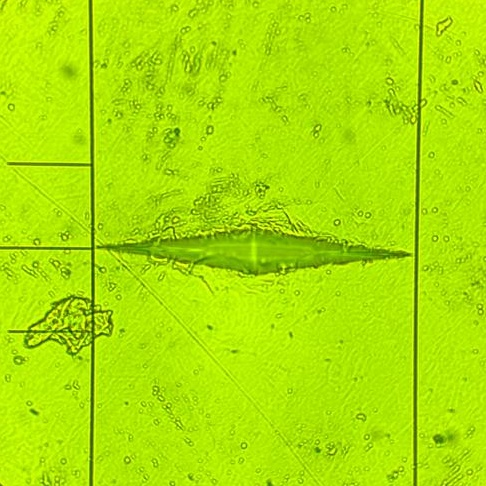
\includegraphics[width=0.80\columnwidth]{Figuras/fig_knoop.jpg}};
\begin{scope}[x={(img.south east)}, y={(img.north west)}]
 % Barra de escala: 50 um = 135.6 px de un recorte de 486 px de ancho => 0.279
 \draw[black, line width=1.6pt] (0.06,0.07) -- (0.339,0.07);
 \node[black, font=\scriptsize, anchor=south] at (0.1995,0.08) {50~\textmu m};
 % Cota de la diagonal mayor (entre las líneas verticales del retículo)
 \draw[black, {Stealth[length=2mm]}-{Stealth[length=2mm]}] (0.187,0.64) -- (0.858,0.64);
 \node[black, font=\scriptsize, anchor=south] at (0.5225,0.65) {$d=120{,}2$~\textmu m};
\end{scope}
\end{tikzpicture}
\caption{Huella Knoop (500~gf, 10~s) sobre la probeta empastillada, vista a través del ocular con el retículo de medición.}
\label{fig:knoop}
\end{figure}

\begin{table}[!t]
\caption{Resultado de microdureza Knoop.}
\label{tab:knoop}
\centering\footnotesize
\begin{tabular}{@{}ccccc@{}}
\toprule
$P$ (gf) & $d_1$ (\textmu m) & $d_2$ (\textmu m) & $\bar{d}$ (\textmu m) & HK\\
\midrule
500 & 120,2 & 120,2 & 120,2 & 492,4\\
\bottomrule
\end{tabular}
\end{table}

\subsection{Comparación entre escalas}
La Tabla~\ref{tab:conv} confronta las mediciones con la carta de conversión \cite{leco}. Los 492,4~HK obtenidos equivalen en la carta de conversión \cite{leco} a $\approx$47~HRC, valor al que la carta asigna 495~HK y 471~HV (una diferencia de apenas 0,53~\% en HK), coherentes con los 47~HRC rotulados en la probeta, lo que valida cruzadamente la microdureza y la medición Rockwell. Estas equivalencias, sin embargo, son empíricas y las de la carta de aceros no deben extenderse al cobre, para el cual la norma tiene tablas propias \cite{astm140}; de hecho, la equivalencia HRB--HRF del cobre se tomó de la sección general de metales no ferrosos de la carta y no de una tabla específica para cobre, por lo que es solo indicativa.

\begin{table}[!t]
\caption{Equivalencias según la carta de conversión.}
\label{tab:conv}
\centering\footnotesize
\begin{tabular}{@{}lll@{}}
\toprule
Medición & Medido & Equivalencia (carta)\\
\midrule
Acero (HRC) & 65,3 HRC & $\approx$832 HV; $\approx$846 HK\\
Probeta (Knoop) & 492 HK & $\approx$47 HRC; $\approx$471 HV\\
Cobre (HRB) & 22,2 HRB & $\approx$70 HRF\\
\bottomrule
\end{tabular}
\end{table}

\subsection{Limitaciones}
Entre las limitaciones están el número reducido de ensayos ($n$ de 4 a 6), la lectura visual en un equipo analógico, la ausencia de verificación con patrón para las escalas B y F, el desconocimiento de la composición y del tratamiento de las probetas, la huella Knoop única y la naturaleza aproximada de las conversiones. Asimismo, respecto a la probeta empastillada, no se contó con información adicional más allá de su rotulado ni se realizó ataque químico para revelar su microestructura; cabe señalar que una etapa isotérmica a 200~\si{\degreeCelsius} queda por debajo de la temperatura $M_s$ estimada para un acero 1045 ($\approx$325~\si{\degreeCelsius}, ecuación de Andrews \cite{andrews}), por lo que el proceso real probablemente correspondió a un temple con revenido bajo más que a un austemperado estricto, si bien la dureza de 47~HRC no basta por sí sola para distinguirlos. Se recomienda verificar el equipo con un patrón en cada escala, aumentar el número de ensayos y emplear al menos cinco huellas Knoop.

% =====================================================================
\section{Conclusiones}
\begin{itemize}
\item La selección de la escala condiciona la validez del ensayo: en el cobre, la escala C no fue válida (aguja con $\approx$2,5 vueltas, $e\approx\SI{0,5}{\milli\metre}$), la B quedó cerca del límite inferior (22,2~HRB) y solo la F entregó una medición confiable ($71{,}8\pm2{,}0$~HRF).
\item El durómetro Wolpert resultó exacto en promedio (error de $-0{,}03$~HRC con el patrón) pero con dispersión apreciable (rango de 2,0~HRC y $s=0{,}82$~HRC), propia de un equipo analógico manual, por lo que conviene verificarlo en cada escala.
\item El acero presentó $65{,}3\pm0{,}5$~HRC (CV~=~0,7~\%), equivalente a $\approx$832~HV, compatible con un acero templado y de revenido bajo.
\item La microdureza Knoop con 500~gf (diagonal de 120,2~\textmu m) fue de 492~HK~0,5 ($\approx$4,8~GPa), consistente con $\approx$47~HRC al convertirla, lo que respalda la coherencia entre ambos métodos en aceros.
\item Las conversiones entre escalas son aproximadas y válidas solo para la familia de materiales con que se construyeron; la calidad de la medición depende de la escala, de la preparación de la superficie y del número de ensayos.
\end{itemize}

\section*{Agradecimientos}
Los autores agradecen al técnico del Laboratorio de Metalografía y al profesor Jhon Jairo Olaya por la orientación durante la práctica.

% =====================================================================
\begin{thebibliography}{99}
\bibitem{callister} W. D. Callister Jr. and D. G. Rethwisch, \emph{Materials Science and Engineering: An Introduction}, 10th ed. Hoboken, NJ, USA: Wiley, 2018.
\bibitem{ashby} M. F. Ashby and D. R. H. Jones, \emph{Engineering Materials 1: An Introduction to Properties, Applications and Design}, 4th ed. Oxford, U.K.: Butterworth-Heinemann/Elsevier, 2012.
\bibitem{tabor} D. Tabor, \emph{The Hardness of Metals}. Oxford, U.K.: Clarendon Press, 1951.
\bibitem{asmhb} ASM International, \emph{ASM Handbook, Vol. 8: Mechanical Testing and Evaluation}. Materials Park, OH, USA: ASM International, 2000.
\bibitem{astm18} \emph{Standard Test Methods for Rockwell Hardness of Metallic Materials}, ASTM E18-24, ASTM International, West Conshohocken, PA, USA, 2024.
\bibitem{iso6508} \emph{Metallic Materials --- Rockwell Hardness Test --- Part 1: Test Method}, ISO 6508-1:2023, 2023.
\bibitem{astm384} \emph{Standard Test Method for Microindentation Hardness of Materials}, ASTM E384-22, ASTM International, West Conshohocken, PA, USA, 2022.
\bibitem{iso4545} \emph{Metallic Materials --- Knoop Hardness Test --- Part 1: Test Method}, ISO 4545-1:2023, 2023.
\bibitem{knoop} F. Knoop, C. G. Peters, and W. B. Emerson, ``A sensitive pyramidal-diamond tool for indentation measurements,'' \emph{J. Res. Natl. Bur. Stand.}, vol. 23, no. 1, 1939.
\bibitem{broitman} E. Broitman, ``Indentation hardness measurements at macro-, micro-, and nanoscale: A critical overview,'' \emph{Tribol. Lett.}, vol. 65, no. 1, Art. no. 23, 2017.
\bibitem{forero} \'A. Forero Mora, \emph{Laboratorio de Metales}, Publicaciones de la Facultad de Ingeniería, Univ. Nacional de Colombia, Bogotá, Colombia.
\bibitem{astm140} \emph{Standard Hardness Conversion Tables for Metals}, ASTM E140-12b(2019)e1, ASTM International, West Conshohocken, PA, USA, 2019.
\bibitem{leco} LECO Corporation, \emph{Hardness Conversion Charts}, St. Joseph, MI, USA. Carta de conversión consultada en el Laboratorio de Metalografía, Univ. Nacional de Colombia, Sede Bogotá, 21 oct. 2026.
\bibitem{gum} \emph{Evaluation of Measurement Data --- Guide to the Expression of Uncertainty in Measurement}, JCGM 100:2008, BIPM, 2008.
\bibitem{andrews} K. W. Andrews, ``Empirical formulae for the calculation of some transformation temperatures,'' \emph{J. Iron Steel Inst.}, vol. 203, pp. 721--727, 1965.
\end{thebibliography}

% =====================================================================
\section*{Anexo A. Cálculos de muestra}
\textbf{Acero.} $\bar{x}=(65{,}1+64{,}9+65{,}0+65{,}0+66{,}0+65{,}6)/6=65{,}27$~HRC; $s=0{,}437$~HRC; $\mathrm{CV}=0{,}67$~\%; $t_{0{,}975,5}=2{,}571$, de modo que $\mathrm{IC}_{95}=2{,}571\cdot0{,}437/\sqrt{6}=\pm0{,}46$~HRC. Profundidad: $e=(100-65{,}27)\cdot0{,}002=0{,}069$~mm; espesor mínimo $10e=0{,}69$~mm.

\textbf{Patrón.} $\bar{x}=79{,}9/4=19{,}975$~HRC; $E=19{,}975-20=-0{,}025$~HRC; $s=0{,}818$~HRC; $t_{0{,}975,3}=3{,}182$, de modo que $\mathrm{IC}_{95}=\pm1{,}30$~HRC.

\textbf{Cobre (F).} $\bar{x}=430{,}7/6=71{,}78$~HRF; $s=1{,}903$~HRF; $\mathrm{IC}_{95}=2{,}571\cdot1{,}903/\sqrt{6}=\pm2{,}00$~HRF. Profundidad: $e=(130-71{,}78)\cdot0{,}002=0{,}116$~mm; $10e=1{,}16$~mm y $15e=1{,}75$~mm.

\textbf{Cobre (B y C).} HRB: $e=(130-22{,}2)\cdot0{,}002=0{,}216$~mm. HRC (descartada): la lectura de 47,15 es la fracción de la tercera vuelta, de modo que el avance fue de $(2+0{,}5285)\cdot100=252{,}85$ unidades y $e\approx252{,}85\cdot0{,}002=0{,}51$~mm.

\textbf{Knoop.} $\mathrm{HK}=14{,}229\cdot0{,}5/(0{,}1202)^2=492{,}4$~kgf/mm$^2$; $\times9{,}80665=4829$~MPa. $b=120{,}2/7{,}11=16{,}9$~\textmu m; profundidad $\approx120{,}2/30{,}5=3{,}9$~\textmu m. Sensibilidad: $\Delta\mathrm{HK}/\mathrm{HK}=2\,\Delta d/d=2(1)/120{,}2=1{,}7$~\%. Límite elástico aproximado: $\sigma_y\approx H/3=4{,}83/3\approx1{,}6$~GPa.

\section*{Anexo B. Registro fotográfico}
\begin{figure*}[!t]
\centering
\begin{minipage}[b]{0.20\textwidth}\centering
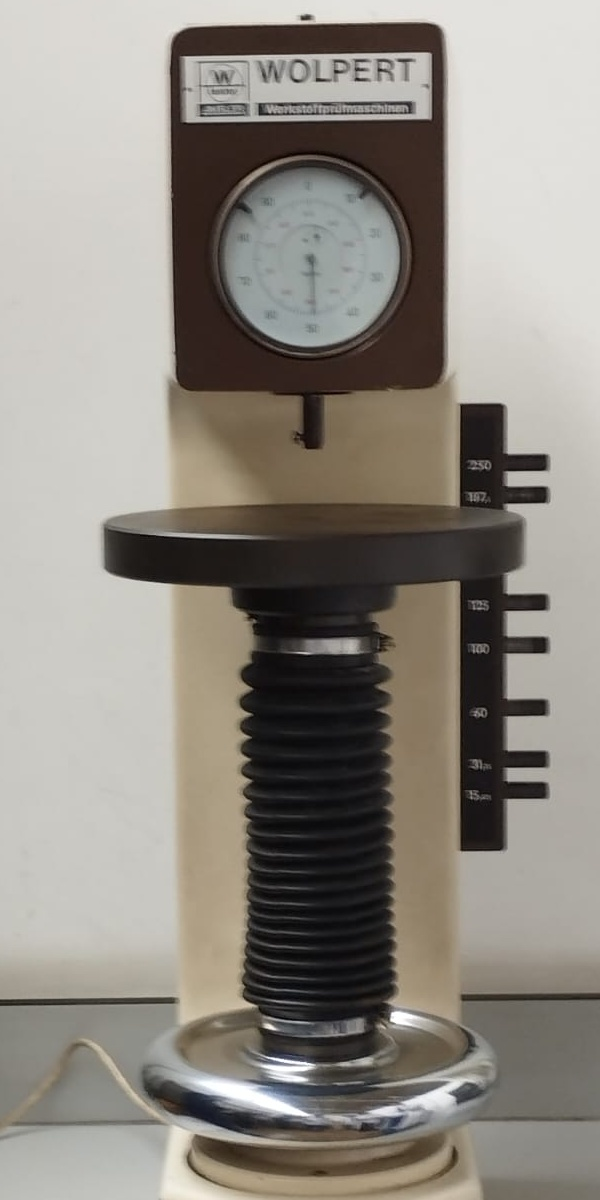
\includegraphics[height=7cm]{Figuras/anexo_wolpert.jpg}\\(a)
\end{minipage}\hfill
\begin{minipage}[b]{0.30\textwidth}\centering
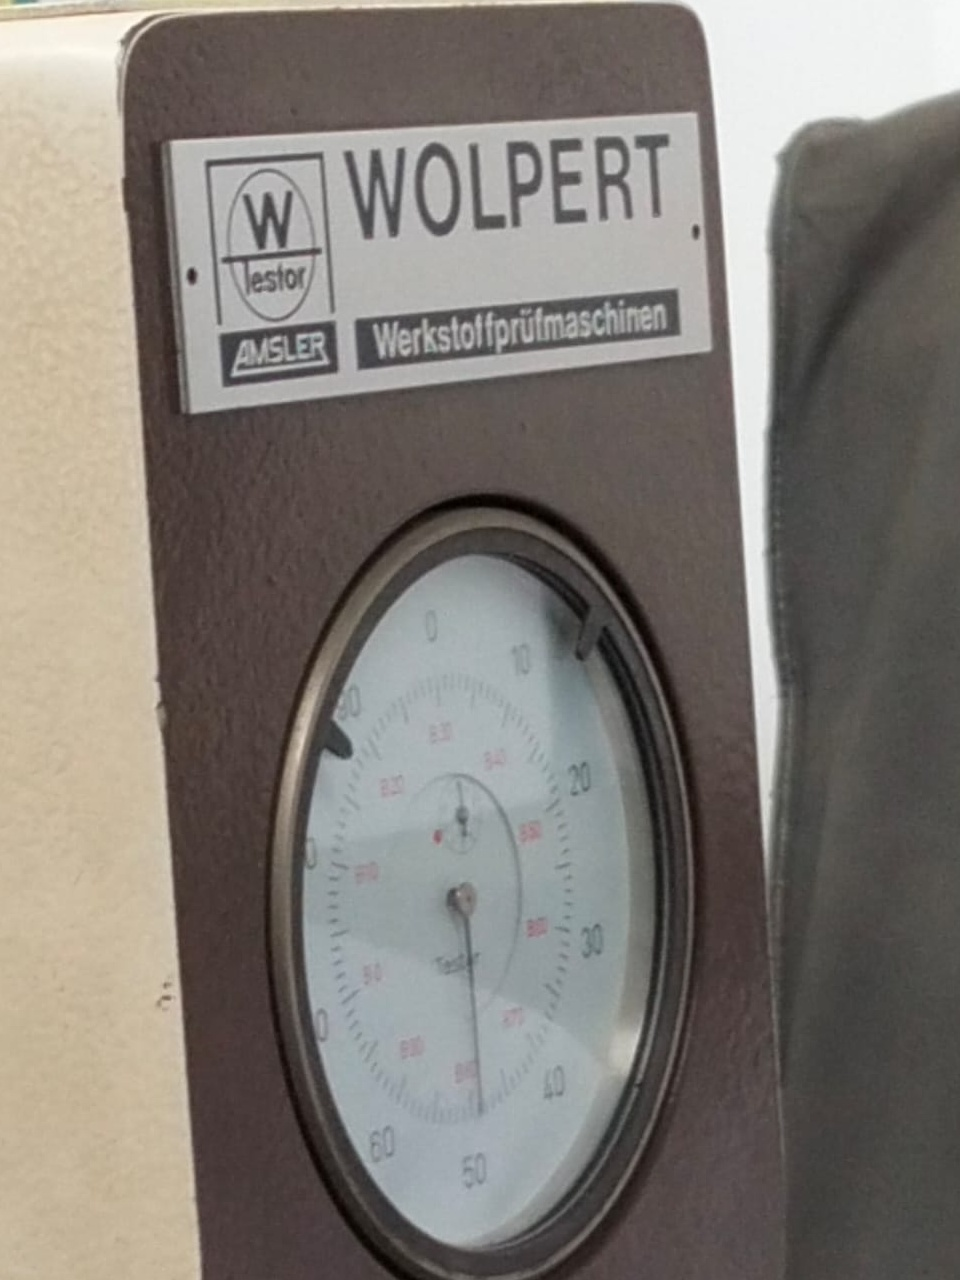
\includegraphics[height=7cm]{Figuras/anexo_caratula.jpg}\\(b)
\end{minipage}\hfill
\begin{minipage}[b]{0.30\textwidth}\centering
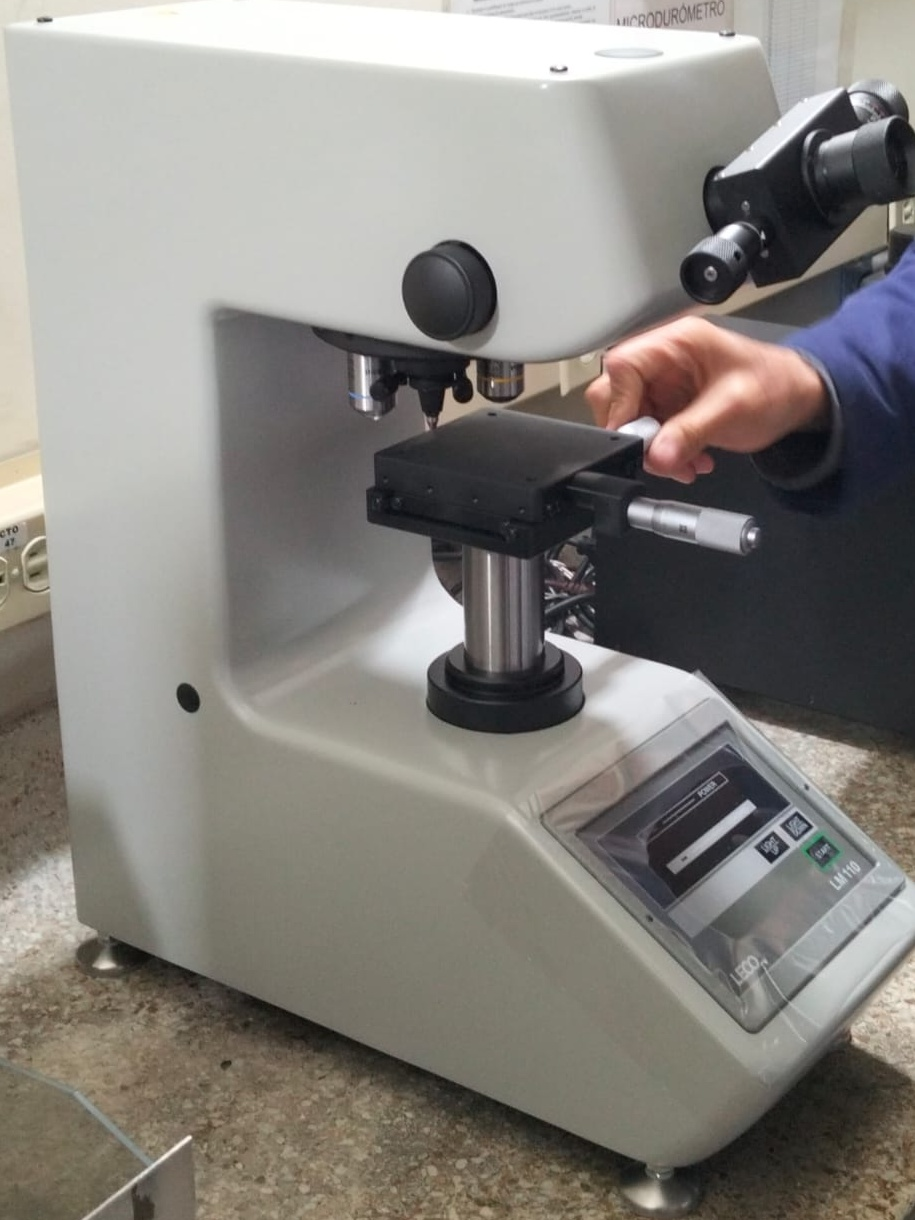
\includegraphics[height=7cm]{Figuras/anexo_leco.jpg}\\(c)
\end{minipage}
\caption{Equipos utilizados: (a) durómetro Wolpert HT~2000, (b) carátula con escalas negra y roja, (c) microdurómetro LECO LM~110.}
\label{fig:anexo1}
\end{figure*}

\begin{figure*}[!t]
\centering
\begin{minipage}[b]{0.28\textwidth}\centering
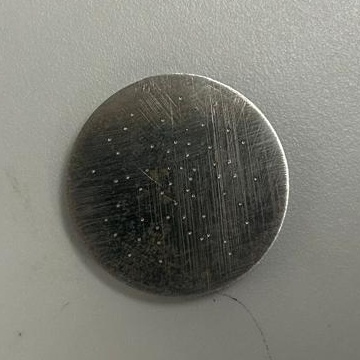
\includegraphics[height=5cm]{Figuras/anexo_disco_acero.jpg}\\(a)
\end{minipage}\hfill
\begin{minipage}[b]{0.28\textwidth}\centering
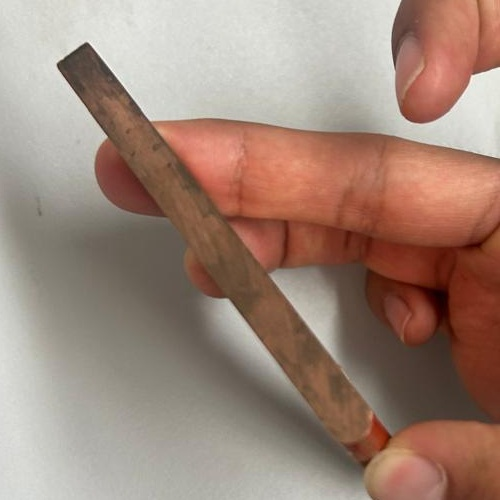
\includegraphics[height=5cm]{Figuras/anexo_barra_cobre.jpg}\\(b)
\end{minipage}\hfill
\begin{minipage}[b]{0.28\textwidth}\centering
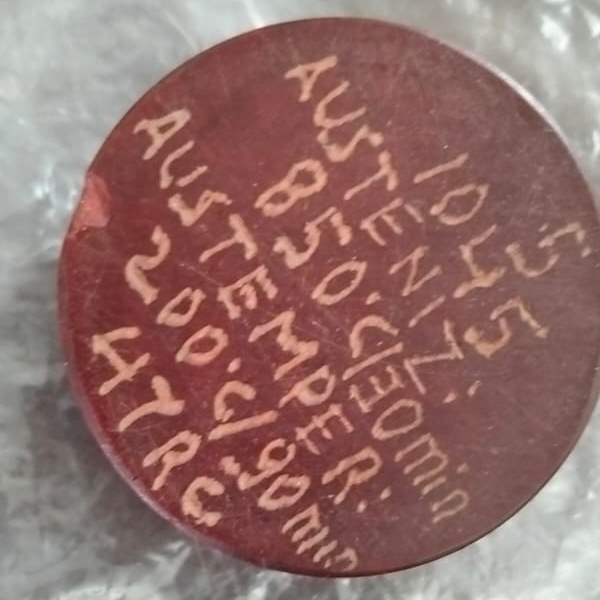
\includegraphics[height=5cm]{Figuras/anexo_baquelita.jpg}\\(c)
\end{minipage}
\caption{Probetas: (a) disco de acero con las huellas Rockwell, (b) barra de cobre con óxido superficial, (c) probeta empastillada en baquelita para microdureza.}
\label{fig:anexo2}
\end{figure*}

\end{document}